\documentclass{article}
\usepackage[utf8]{inputenc}
\usepackage{tikz}
\usepackage{wrapfig}

\begin{document}

\section{Autómata Finito Determinista}

\begin{wrapfigure}{l}{0.6\textwidth}
\centering
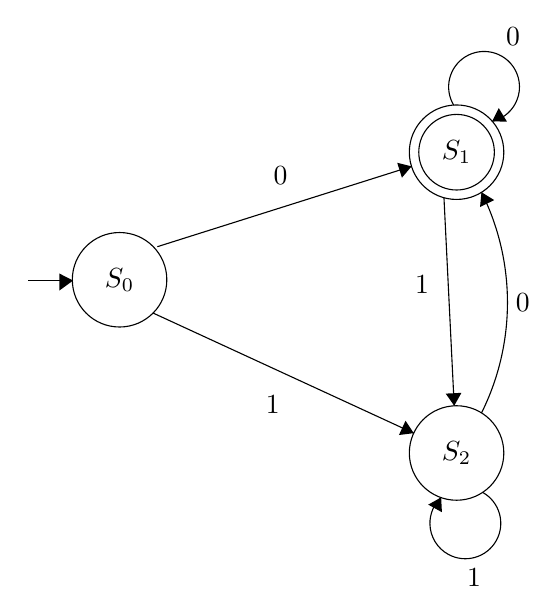
\begin{tikzpicture}[scale=0.2]
\tikzstyle{every node}+=[inner sep=0pt]
\draw [black] (16.3,-28.1) circle (3);
\draw (16.3,-28.1) node {$S_0$};
\draw [black] (37.7,-20) circle (3);
\draw (37.7,-20) node {$S_1$};
\draw [black] (37.7,-20) circle (2.4);
\draw [black] (37.7,-39.1) circle (3);
\draw (37.7,-39.1) node {$S_2$};
\draw [black] (18.7,-26) -- (34.84,-20.9);
\draw (27,-21.5) node [left] {$0$};
\fill [black] (34.84,-20.9) -- (33.93,-20.67) -- (34.23,-21.62);
\draw [black] (18.4,-30.2) -- (34.98,-37.84);
\draw (26.5,-36) node [left] {$1$};
\fill [black] (34.98,-37.84) -- (34.46,-37.05) -- (34.04,-37.96);
\draw [black] (37.521,-17.017) arc (211.17258:-76.82742:2.25);
\draw (41.29,-13.26) node [above] {$0$};
\fill [black] (39.96,-18.04) -- (40.9,-18.06) -- (40.38,-17.2);
\draw [black] (36.9,-22.9) -- (37.55,-36.1);
\draw (35.5,-29) node [above] {$1$};
\fill [black] (37.55,-36.1) -- (38.01,-35.28) -- (37.01,-35.33);
\draw [black] (39.284,-22.542) arc (26.46493:-26.46493:15.725);
\fill [black] (39.28,-22.54) -- (39.19,-23.48) -- (40.09,-23.04);
\draw (41.43,-29.55) node [right] {$0$};
\draw [black] (39.344,-41.595) arc (61.1203:-226.8797:2.25);
\draw (38.81,-46.39) node [below] {$1$};
\fill [black] (36.72,-41.92) -- (35.9,-42.38) -- (36.77,-42.86);
\fill [black] (13.35,-28.15) -- (12.47,-27.7) -- (12.47,-28.79) --(13.35,-28.15);
\draw [black] (10.5,-28.15) -- (13.35,-28.15);
\end{tikzpicture}
\end{wrapfigure}
El último dígito de un número binario representa el residuo que el número deja al ser dividido entre dos. Por lo que para que un número binario sea par debe terminar en $0$.\\
\\
\\
\\
\\
\\
\\
\\
\\
\\
\\
\\
\\
\section{Expresión regular}
Como ya lo establecimos anteriormente, las cadenas o expresiones regulares que este autómata acepta finalizan en $0$. Ahora, por los dos caminos que una cadena puede tomar al ingresar al autómata, podemos notar intuitivamente que las expresiones regulares deben tener la forma $(0|1)^{+}0$ o $(0|1)(0|1)^*0$. Al menos estamos seguros de que inicia con $(0|1)$ y termina con cero. Ahora, observemos que cuando una subcadena llega a $S_2$ de nuevo puede tomar dos formas, o el siguiente caracter en la cadena puede ser $0$ o $1$; lo mismo sucede con $S_1$. También observamos que $S_1$ y $S_2$ están enciclados por lo que nuestra expresión regular puede tomar las formas que ya establecimos\footnote{Probé varias veces hacer un procedimiento más \textit{formal} para encontrar la expresión regular pero no me convencían. Además las probaba para ver si sí me daban el autómata. La única que me funcionó fueron estas y esas ese fue el razonamiento que utilicé}. 
\end{document}
